\documentclass[11pt,a4paper]{scartcle}
\usepackage[utf8]{inputenc}
\usepackage[T1]{fontenc}
\usepackage[ngerman]{babel}
\usepackage{amsmath}
\usepackage{amsfonts}
\usepackage{amssymb}
\usepackage{graphicx}
\begin{document}

\hypertarget{bauhaus-university-sose2021-iaor-assignment-1}{%
\section{Bauhaus University SoSe2021 IAOR Assignment
1}\label{bauhaus-university-sose2021-iaor-assignment-1}}

\hypertarget{groip-j-team-members}{%
\subsection{Groip J Team members}\label{groip-j-team-members}}

Yen Lung Chen
Martin 119982 Henrik Leisdon, 118334 \#\# Topic * Image
enhancement * Derivation of a binary mask by thresholding * Refinement
of the mask by using morphological operators \#\#Task A

\hypertarget{shortly-describe-the-characteristics-of-the-histogram}{%
\subsubsection{Shortly describe the characteristics of the
histogram}\label{shortly-describe-the-characteristics-of-the-histogram}}
Histogram is a graph showing the number of pixels in an image(y axis) at each different intensity value(x axis) found in that image. Figure 1:
\begin{table}
\begin{tabular}{|c|c|}
	\hline
Original Image & Image with enhanced contrast \\
	\hline
		\begin{figure}
		\centering
		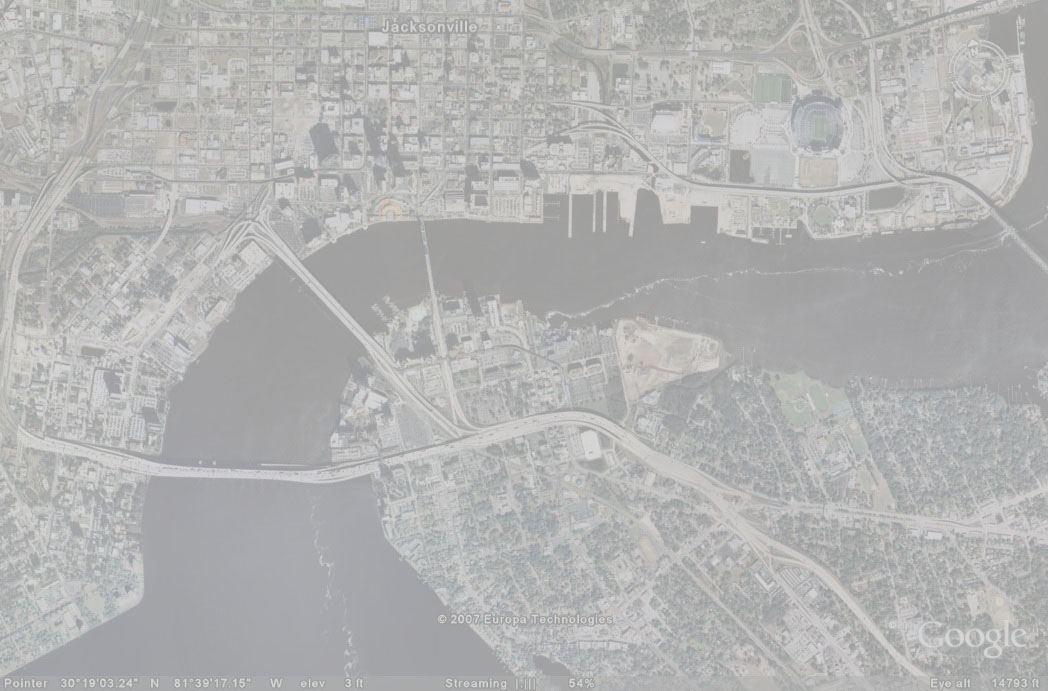
\includegraphics[width=0.5\linewidth]{input_sat_image.jpg}
		\caption{histogram}
	\end{figure}  &  \begin{figure}
	\centering
	\includegraphics[width=0.5\linewidth]{https://user-images.githubusercontent.com/39960241/115701181-cfe85180-a367-11eb-8f5d-32471cbe1fcb.jpg}
	\caption{enhancementHistogram}
\end{figure}
 \\
	\hline
	\begin{figure}
		\centering
		\includegraphics[width=0.5\linewidth]{https://user-images.githubusercontent.com/39960241/115700910-80098a80-a367-11eb-8cc2-1180358b52ca.jpg}
		\caption{actual image corresponding to the histogram}
	\end{figure} &  \begin{figure}
	\centering
	\includegraphics[width=0.5\linewidth]{https://user-images.githubusercontent.com/39960241/115701343-fc03d280-a367-11eb-9595-d579483f65f2.jpg}
	\caption{enhancedImage}
\end{figure} \\
	\hline
\end{tabular}
\end{table}

%\begin{figure}
%\centering
%\includegraphics{https://user-images.githubusercontent.com/39960241/115700026-8fd49f00-a366-11eb-9840-db4ae003fcbe.jpg}
%\caption{histogram}
%\end{figure}

%\begin{figure}
%\centering
%\includegraphics{https://user-images.githubusercontent.com/39960241/115700910-80098a80-a367-11eb-8cc2-1180358b52ca.jpg}
%\caption{actual image corresponding to the histogram}
%\end{figure}
\hypertarget{shortly-describe-the-differences-to-the-initial-histogram-after-enhancement}{%
\subsubsection{Shortly describe the differences to the initial histogram
after
enhancement}\label{shortly-describe-the-differences-to-the-initial-histogram-after-enhancement}}
The figure 1 shows a low-contrast image as the the values of x axis in intensity hitogram are only distrbuted in a certain range. To improve the visual quality of the image, One technique of image enhancement is contrast stretching on histogram where the image has to use the full intensity range to display the maximum contrast. Contrast stretching takes an image in which the intensity values span the full intensity range as the figure 3 and 4 shown.
%\begin{figure}
%\centering
%\includegraphics{https://user-images.githubusercontent.com/39960241/115701181-cfe85180-a367-11eb-8f5d-32471cbe1fcb.jpg}
%\caption{enhancementHistogram}
%\end{figure}
%
%\begin{figure}
%\centering
%\includegraphics{https://user-images.githubusercontent.com/39960241/115701343-fc03d280-a367-11eb-9595-d579483f65f2.jpg}
%\caption{enhancedImage}
%\end{figure}

\hypertarget{task-b}{%
\subsection{Task B}\label{task-b}}

\hypertarget{different-tresholds}{%
\subsubsection{Different tresholds}\label{different-tresholds}}

The resulting treshold by graytresh is 0.4353 When we set a manuel treshold of 30, there is a highlighted spot in the bottom center of the
image. Therefore we compared the treshold of 0.4 and 0.5. Because the spot in the river is so bright, that if the treshold is to high, the rest of the city is also in the region of interest (ROI). When
the treshold is too low, not the whole river is in the ROI. Therefore we decided to use the resulting treshold of the function \texttt{graytresh}.

\begin{tabular}{|c|c|}
	\hline
	0.3 &  0.4\\
	\hline
	\begin{figure}
		\centering
		\includegraphics[width=0.5\linewidth]{./img/treshold_0_30.jpg}
	\end{figure}
	&  \begin{figure}
		\centering
		\includegraphics[width=0.5\linewidth]{./img/treshold_0_40.jpg}
	\end{figure}\\
	\hline
	0.5 &  \\
	\hline
	\begin{figure}
		\centering
		\includegraphics[width=0.5\linewidth]{./img/treshold_0_50.jpg}
	\end{figure} &  \\
	\hline
\end{tabular}



%\begin{figure}
%	\centering
%\includegraphics[width=0.5\linewidth]{https://github.com/henrik-leisdon/buw_IAOR/blob/20cfede4e657713343a9bfb117d0e4f9333fcb0b/img/treshold_0_30.jpg}
%\end{figure}
%
%
%\begin{figure}
%	\centering
%\includegraphics[width=0.5\linewidth]{https://github.com/henrik-leisdon/buw_IAOR/blob/20cfede4e657713343a9bfb117d0e4f9333fcb0b/img/treshold_0_40.jpg}
%\end{figure}
%
%\begin{figure}
%	\centering
%\includegraphics[width=0.5\linewidth]{https://github.com/henrik-leisdon/buw_IAOR/blob/20cfede4e657713343a9bfb117d0e4f9333fcb0b/img/treshold_0_50.jpg}
%\end{figure}

\hypertarget{different-graytreshoptions}{%
\subsubsection{Different
grayTreshOptions}\label{different-graytreshoptions}}

Also we tried different algorithms of the \texttt{graytresh}-function

\begin{tabular}{|c|c|}
	\hline
	Otsu &  Mean\\
	\hline
	\begin{figure}
		\centering
		\includegraphics[width=0.5\linewidth]{./img/Otsu.jpg}
	\end{figure} &  \begin{figure}
	\centering
	\includegraphics[width=0.5\linewidth]{./img/mean.jpg}
\end{figure}\\
	\hline
	Moments &  \\
	\hline
	\begin{figure}
		\centering
		\includegraphics[width=0.5\linewidth]{./img/moments.jpg}
	\end{figure} &  \\
	\hline
\end{tabular}

%\begin{figure}
%	\centering
%\includegraphics{https://github.com/henrik-leisdon/buw_IAOR/blob/20cfede4e657713343a9bfb117d0e4f9333fcb0b/img/Otsu.jpg}
%\end{figure}
%\begin{figure}
%	\centering
%	\includegraphics{https://github.com/henrik-leisdon/buw_IAOR/blob/20cfede4e657713343a9bfb117d0e4f9333fcb0b/img/mean.jpg}
%\end{figure}
%\begin{figure}
%	\centering
%\includegraphics{https://github.com/henrik-leisdon/buw_IAOR/blob/20cfede4e657713343a9bfb117d0e4f9333fcb0b/img/moments.jpg}
%\end{figure}
By comparing these images we decided to use the Otsu algorithm, because the ROI fitted the best for our needs.

\hypertarget{task-c}{%
\subsection{Task C}\label{task-c}}

\hypertarget{why-did-we-decide-to-diamond-structure-element}{%
\subsubsection[width=0.5\linewidth]{Why did we decide to diamond structure element?}\label{why-did-we-decide-to-diamond-structure-element}}

Since structuring element would greatly affect the edge of the ROI with an urban bird-view image given, we found better result and perception with diamond structure element.

\begin{figure}
\centering
\includegraphics[width=0.5\linewidth]{https://user-images.githubusercontent.com/39960241/116009590-ce927f80-a61a-11eb-9028-e06dfe1ae124.jpg}
\caption{finalOverlay}
\end{figure}

\begin{verbatim}
  0  0  0  0  0  1  0  0  0  0  0
  0  0  0  0  1  1  1  0  0  0  0
  0  0  0  1  1  1  1  1  0  0  0
  0  0  1  1  1  1  1  1  1  0  0
  0  1  1  1  1  1  1  1  1  1  0
  1  1  1  1  1  1  1  1  1  1  1
  0  1  1  1  1  1  1  1  1  1  0
  0  0  1  1  1  1  1  1  1  0  0
  0  0  0  1  1  1  1  1  0  0  0
  0  0  0  0  1  1  1  0  0  0  0
  0  0  0  0  0  1  0  0  0  0  0
\end{verbatim}

\begin{figure}
\centering
\includegraphics[width=0.5\linewidth]{https://user-images.githubusercontent.com/39960241/116009695-64c6a580-a61b-11eb-9be3-569aa6ba2380.jpg}
\caption{finalOverlayWithDisk}
\end{figure}

\begin{verbatim}
  0  0  0  0  0  1  0  0  0  0  0
  0  0  1  1  1  1  1  1  1  0  0
  0  1  1  1  1  1  1  1  1  1  0
  0  1  1  1  1  1  1  1  1  1  0
  0  1  1  1  1  1  1  1  1  1  0
  1  1  1  1  1  1  1  1  1  1  1
  0  1  1  1  1  1  1  1  1  1  0
  0  1  1  1  1  1  1  1  1  1  0
  0  1  1  1  1  1  1  1  1  1  0
  0  0  1  1  1  1  1  1  1  0  0
  0  0  0  0  0  1  0  0  0  0  0
\end{verbatim}

\hypertarget{effect-of-the-size-of-structuring-element}{%
\subsubsection{Effect of the size of  element}\label{effect-of-the-size-of-structuring-element}}

The bigger the structuring element is, less details of ROI or noises can be revealed. \#\#\# Are the results satisfactory? What are the  limitations of this approach for separating background and foreground? Overall we were happy with the result, most of the ROI(the river) was revealed. However there are areas of urban location were taken as ROI, one of the limitations of morphological filter approach is that it require trail-and-error step to have desired outcome.

\hypertarget{significant-difference-with-respect-to-quality-of-the-results-for-the-different-input-images}{%
\subsubsection{Significant difference with respect to quality of the results for the different input images?}\label{significant-difference-with-respect-to-quality-of-the-results-for-the-different-input-images}}

\begin{figure}
\centering
\includegraphics[width=0.5\linewidth]{https://user-images.githubusercontent.com/39960241/116010437-35199c80-a61f-11eb-922e-cfca10c05c15.jpg}
\caption{secondImage}
\end{figure}

\begin{figure}
\centering
\includegraphics[width=0.5\linewidth]{https://user-images.githubusercontent.com/39960241/116010439-3ea30480-a61f-11eb-9d0a-b8f8b5fba088.jpg}
\caption{secondImageFinalOverlay}
\end{figure}

In the second input image we are interested in the fields, and without changing the variables the accuracy of ROI is reduced.

source image1:
https://i.pinimg.com/originals/bc/91/af/bc91af8974e84b7e4897eb52b8ddd3ec.jpg
source image2:
https://c0.wallpaperflare.com/preview/1003/50/552/bird-s-eye-view-photography-of-river-in-city.jpg

In the third we are interested in the water. But due to the different water colors (light and shadow) and the similarities between the foreground and background for the algorithm it is very hard to evaluate. 
\begin{figure}
	\centering
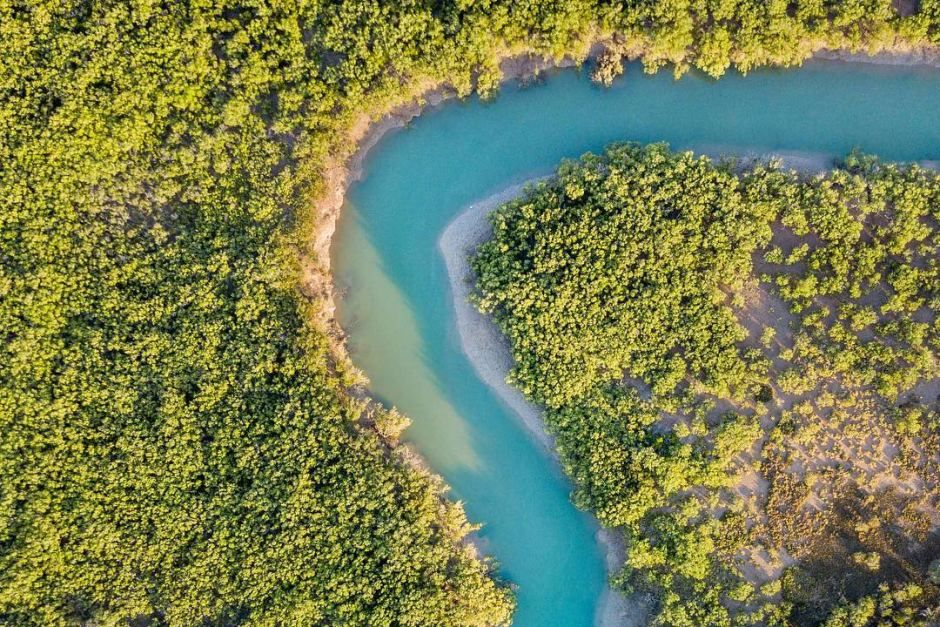
\includegraphics[width=0.5\linewidth]{https://github.com/henrik-leisdon/buw_IAOR/blob/16818f5c02d2ae1437aa297a53f92b9d8e40f480/image1.jpg}
\end{figure}
After inversion, the water/our foreground is detected in the most parts
of the image but, in the shadow areas at the top and bottom of the water
and also at the transition between foreground and background there are
no clear edges. COMMENT to me (henrik): add the final images instead of
the binary!!!
\begin{figure}
	\centering
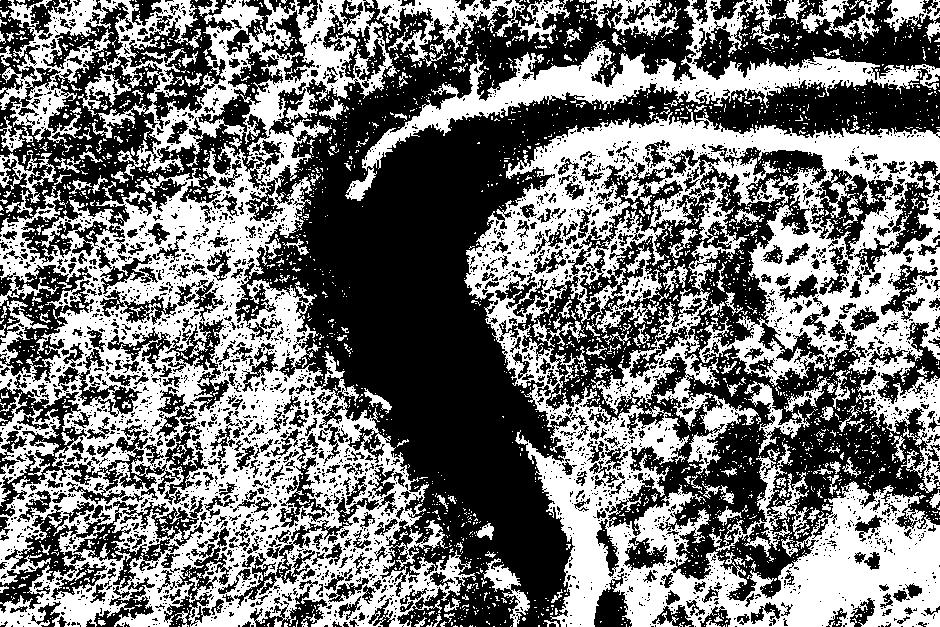
\includegraphics[width=0.5\linewidth]{https://github.com/henrik-leisdon/buw_IAOR/blob/16818f5c02d2ae1437aa297a53f92b9d8e40f480/binaryImage1.jpg}
\end{figure}
In the fourth image we are gain interested in the water. Here it is a
bit clearer because the color difference between the foreground and
background is more clear.
\begin{figure}
	\centering
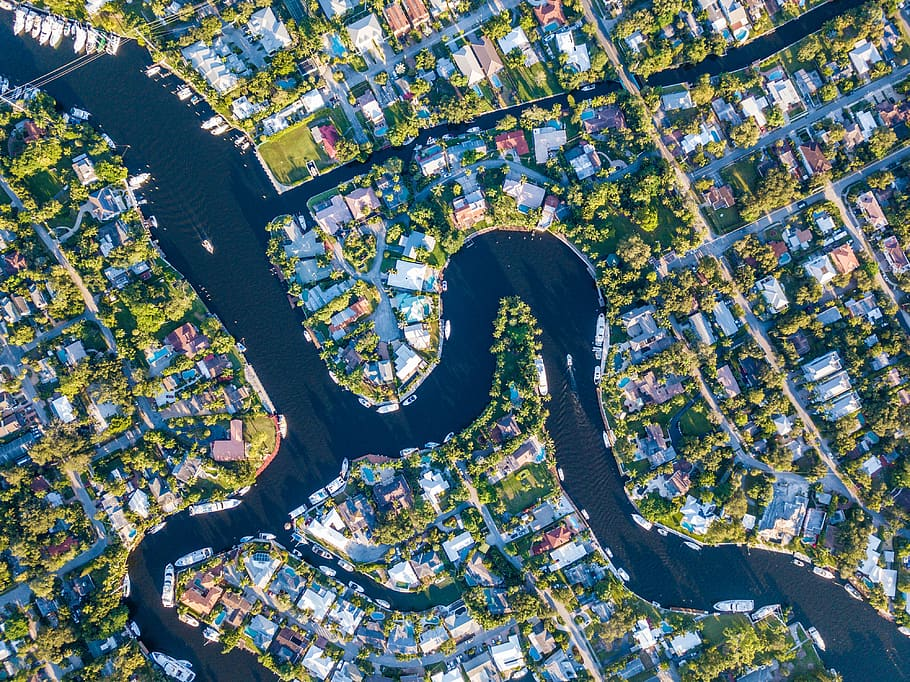
\includegraphics[width=0.5\linewidth]{https://github.com/henrik-leisdon/buw_IAOR/blob/16818f5c02d2ae1437aa297a53f92b9d8e40f480/image2.jpg}
\end{figure}
But again the difference between blue and green is really hard to distinguish. COMMENT to me (henrik): add the final images instead of the binary!!!
\begin{figure}
	\centering
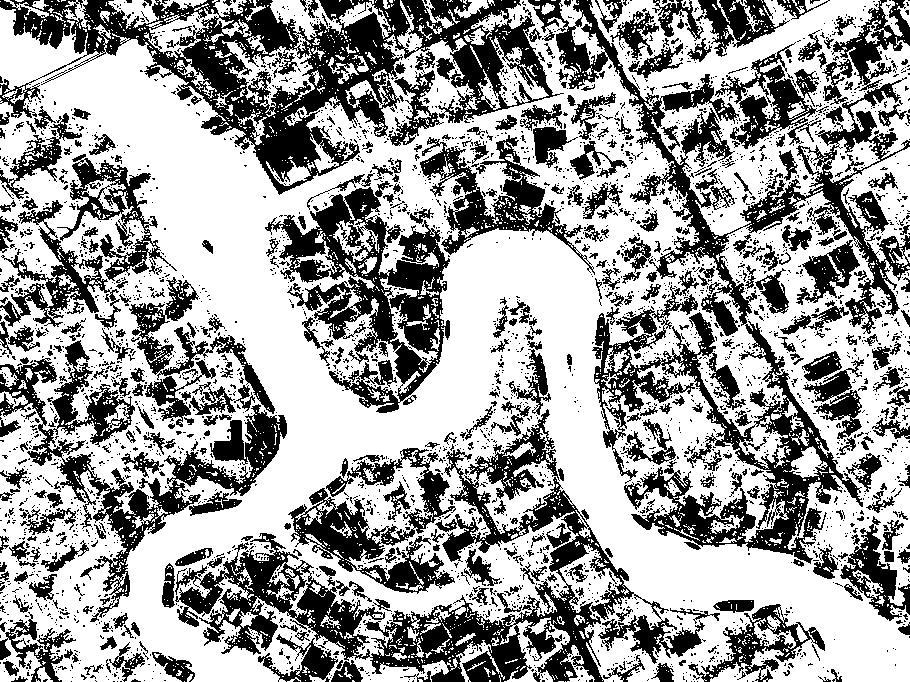
\includegraphics[width=0.5\linewidth]{https://github.com/henrik-leisdon/buw_IAOR/blob/16818f5c02d2ae1437aa297a53f92b9d8e40f480/binaryImage2.jpg}
\end{figure}
\end{document}